\section{Results}
The dependent variables were selection time and the number of clutches.

\subsection{Selection Time}
Selection time is the time between each subsequent target selection. This means that the first target the participants selects for each Transfer Function is not included in the results. Outliers for trials over 20 seconds were removed from the data.

\begin{figure}[h]
    \centering
    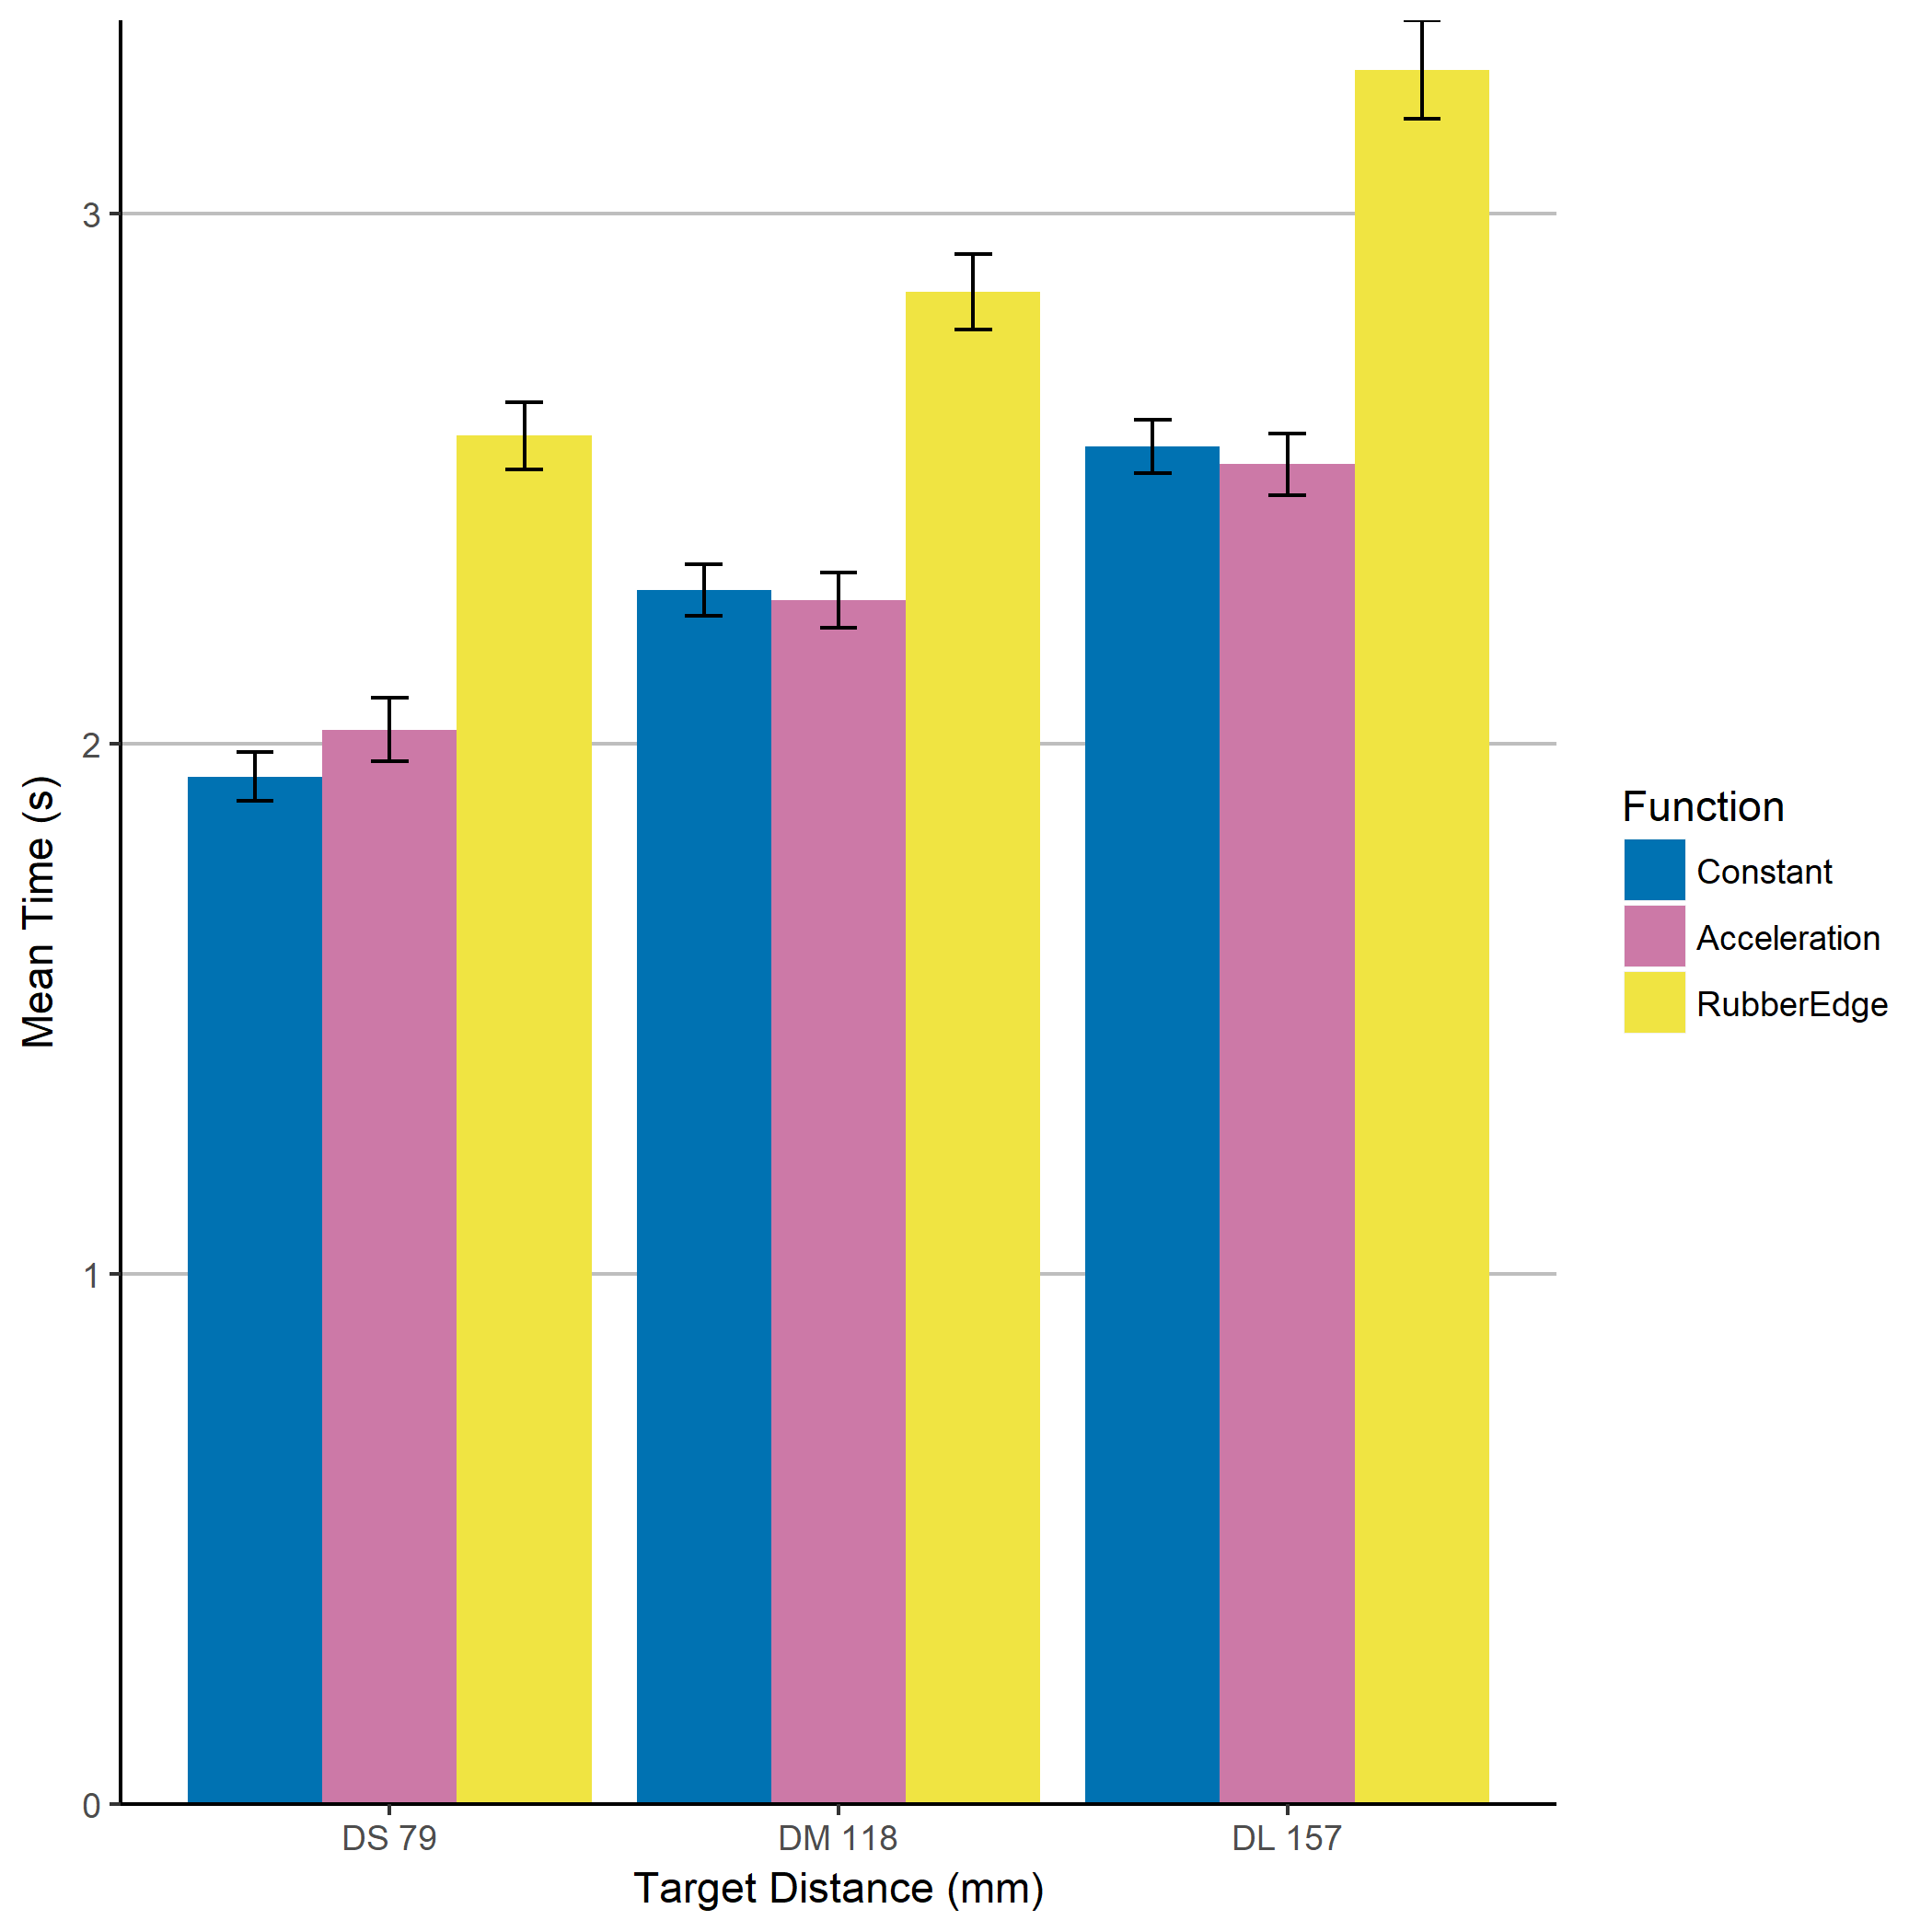
\includegraphics[width=0.9\columnwidth]{selection-time}
    \caption{Selection Time, Transfer Function x Distance Interaction}
    \label{fig:selection-time}
\end{figure}

Repeated measures analysis of variance using Mauchly's Test for Sphericity, showed that the order of Transfer Functions presented to the participant had no significant effect on movement time, so there was no significant asymmetric skill transfer, this indicated that the within-subjects design was appropriate. There was a significant main effect for the for the Transfer Function on selection time (F$_{2,12}$ = 10.3, p < 0.005) with the Constant and Acceleration outperforming the RubberEdge Transfer Function by 21.8\%, this can be seen across all distances in Figure \ref{fig:selection-time}. There was also a significant main effect for Distance (F$_{2,12}$ = 30.8, p < 0.0001) on selection time. The interaction between Transfer Function x Distance was not significant (F$_{2,24}$ = 0.70, p = 0.59). Therefore we cannot accept \textbf{H2}.

Pair-wise comparisons using Bonferroni found that there was a significant difference between RubberEdge and the Constant and Acceleration Transfer Functions. Another pair-wise test also found a significant difference between each distance (D$_S$, D$_M$, D$_L$)

\subsection{Fitts' Law Analysis}

\begin{figure}[h]
    \centering
    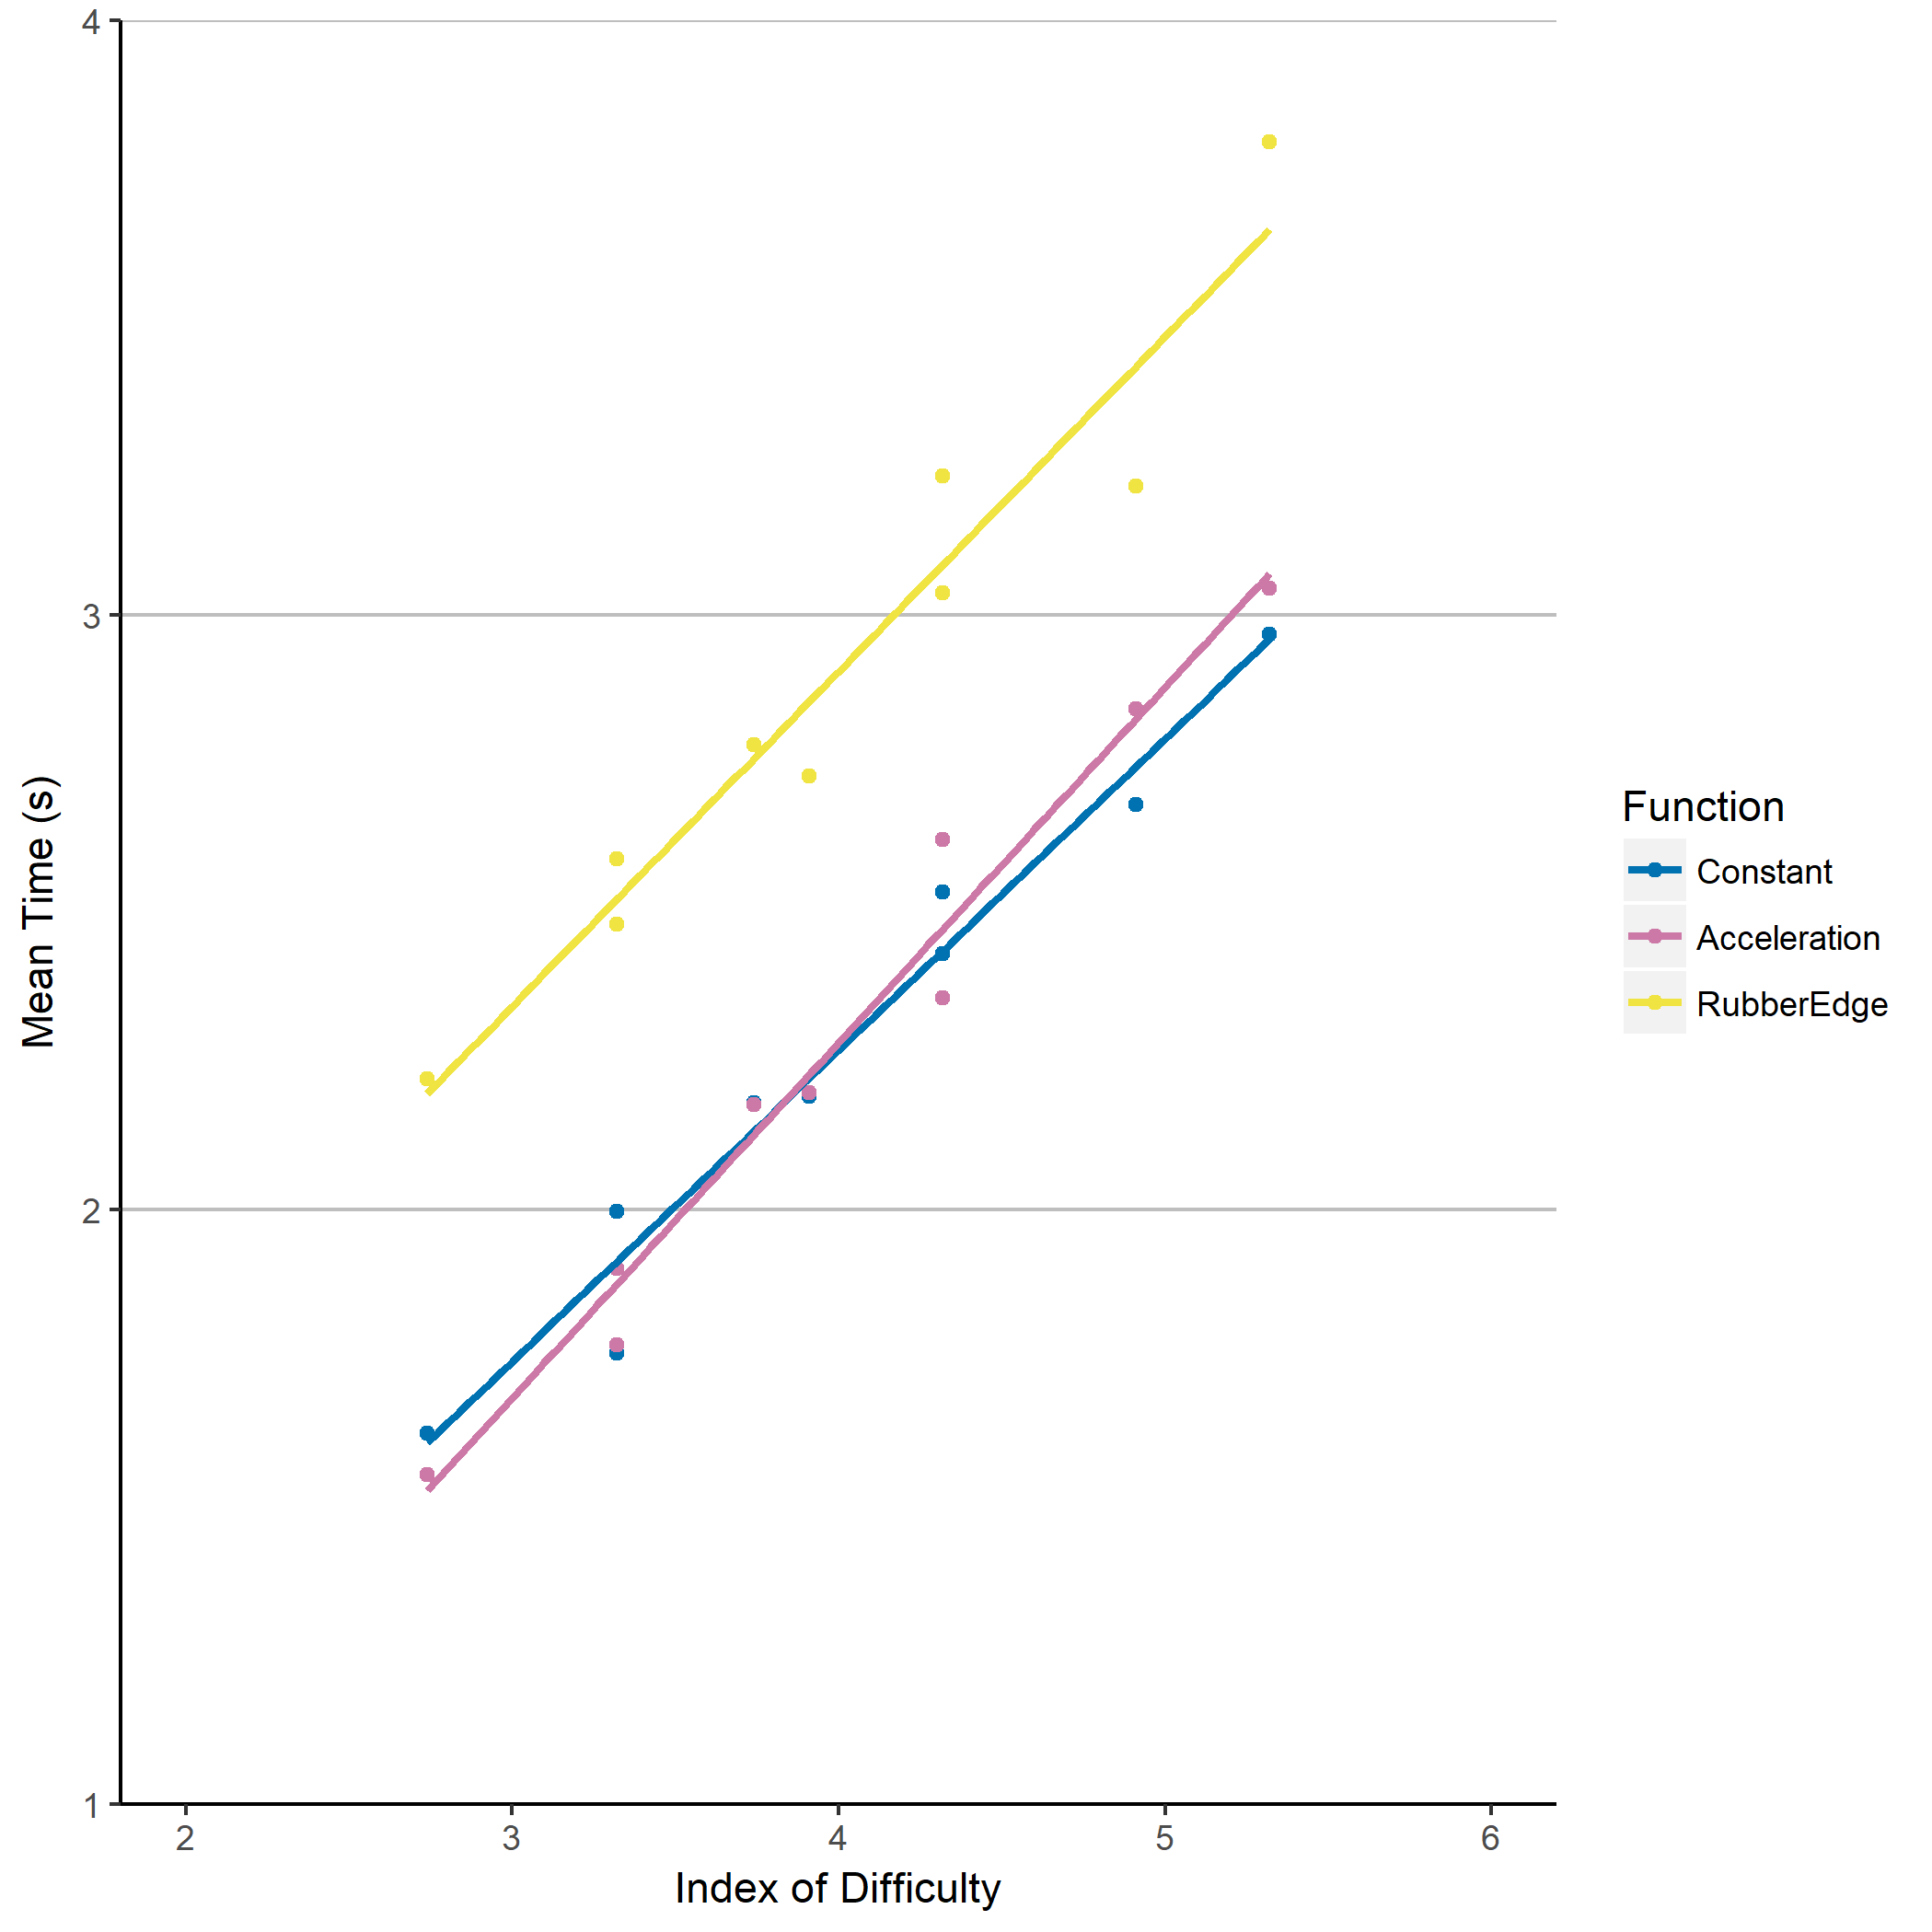
\includegraphics[width=0.9\columnwidth]{fitts}
    \caption{A comparison between the Index of difficulty and mean time, between different transfer functions.}
    \label{fig:fitts}
\end{figure}

A significant difference for Fitts' law between distances was not found (Figure \ref{fig:fitts}). Whereas the previous study\cite{Casiez2007RubberEdge} found that the distance had a significant effect for indexes of the same difficulty. Why the results found in this study differ, is likely because the distances measured against in the previous study were much larger, 172, 344, 688mm. Compared to 79, 118, 157mm for this study. The reason that smaller distances were chosen is that they align closer to distances that users are likely to demonstrate on a laptop device. Specifically, 157mm was around the limit for the distance from the centre point of the laptop screen to the upper or lower edge, see section \ref{section:apparatus} for details about the laptop used. 

\begin{table}[h]
\centering
{\rowcolors{2}{gray!30}{lightgray!30}
\begin{tabular}{ l r r r } 
 Function & $a$ & $b$ & $r^2$ \\ 
 \hline
 Constant & 0.20 & 0.52 & 0.99 \\ 
 Acceleration & -0.08 & 0.59 & 0.99 \\ 
 RubberEdge & 0.64 & 0.56 & 0.95 \\
 \hline
 \end{tabular}
}
\vspace{0.5cm}
 \caption{Fitts' Law regression values for different transfer functions, where $a$ is the intercept of the regression line, $b$ is the slope, $r^2$ is the fitness.}
\label{table:fitts}
\end{table}

\begin{figure}[h]
    \centering
    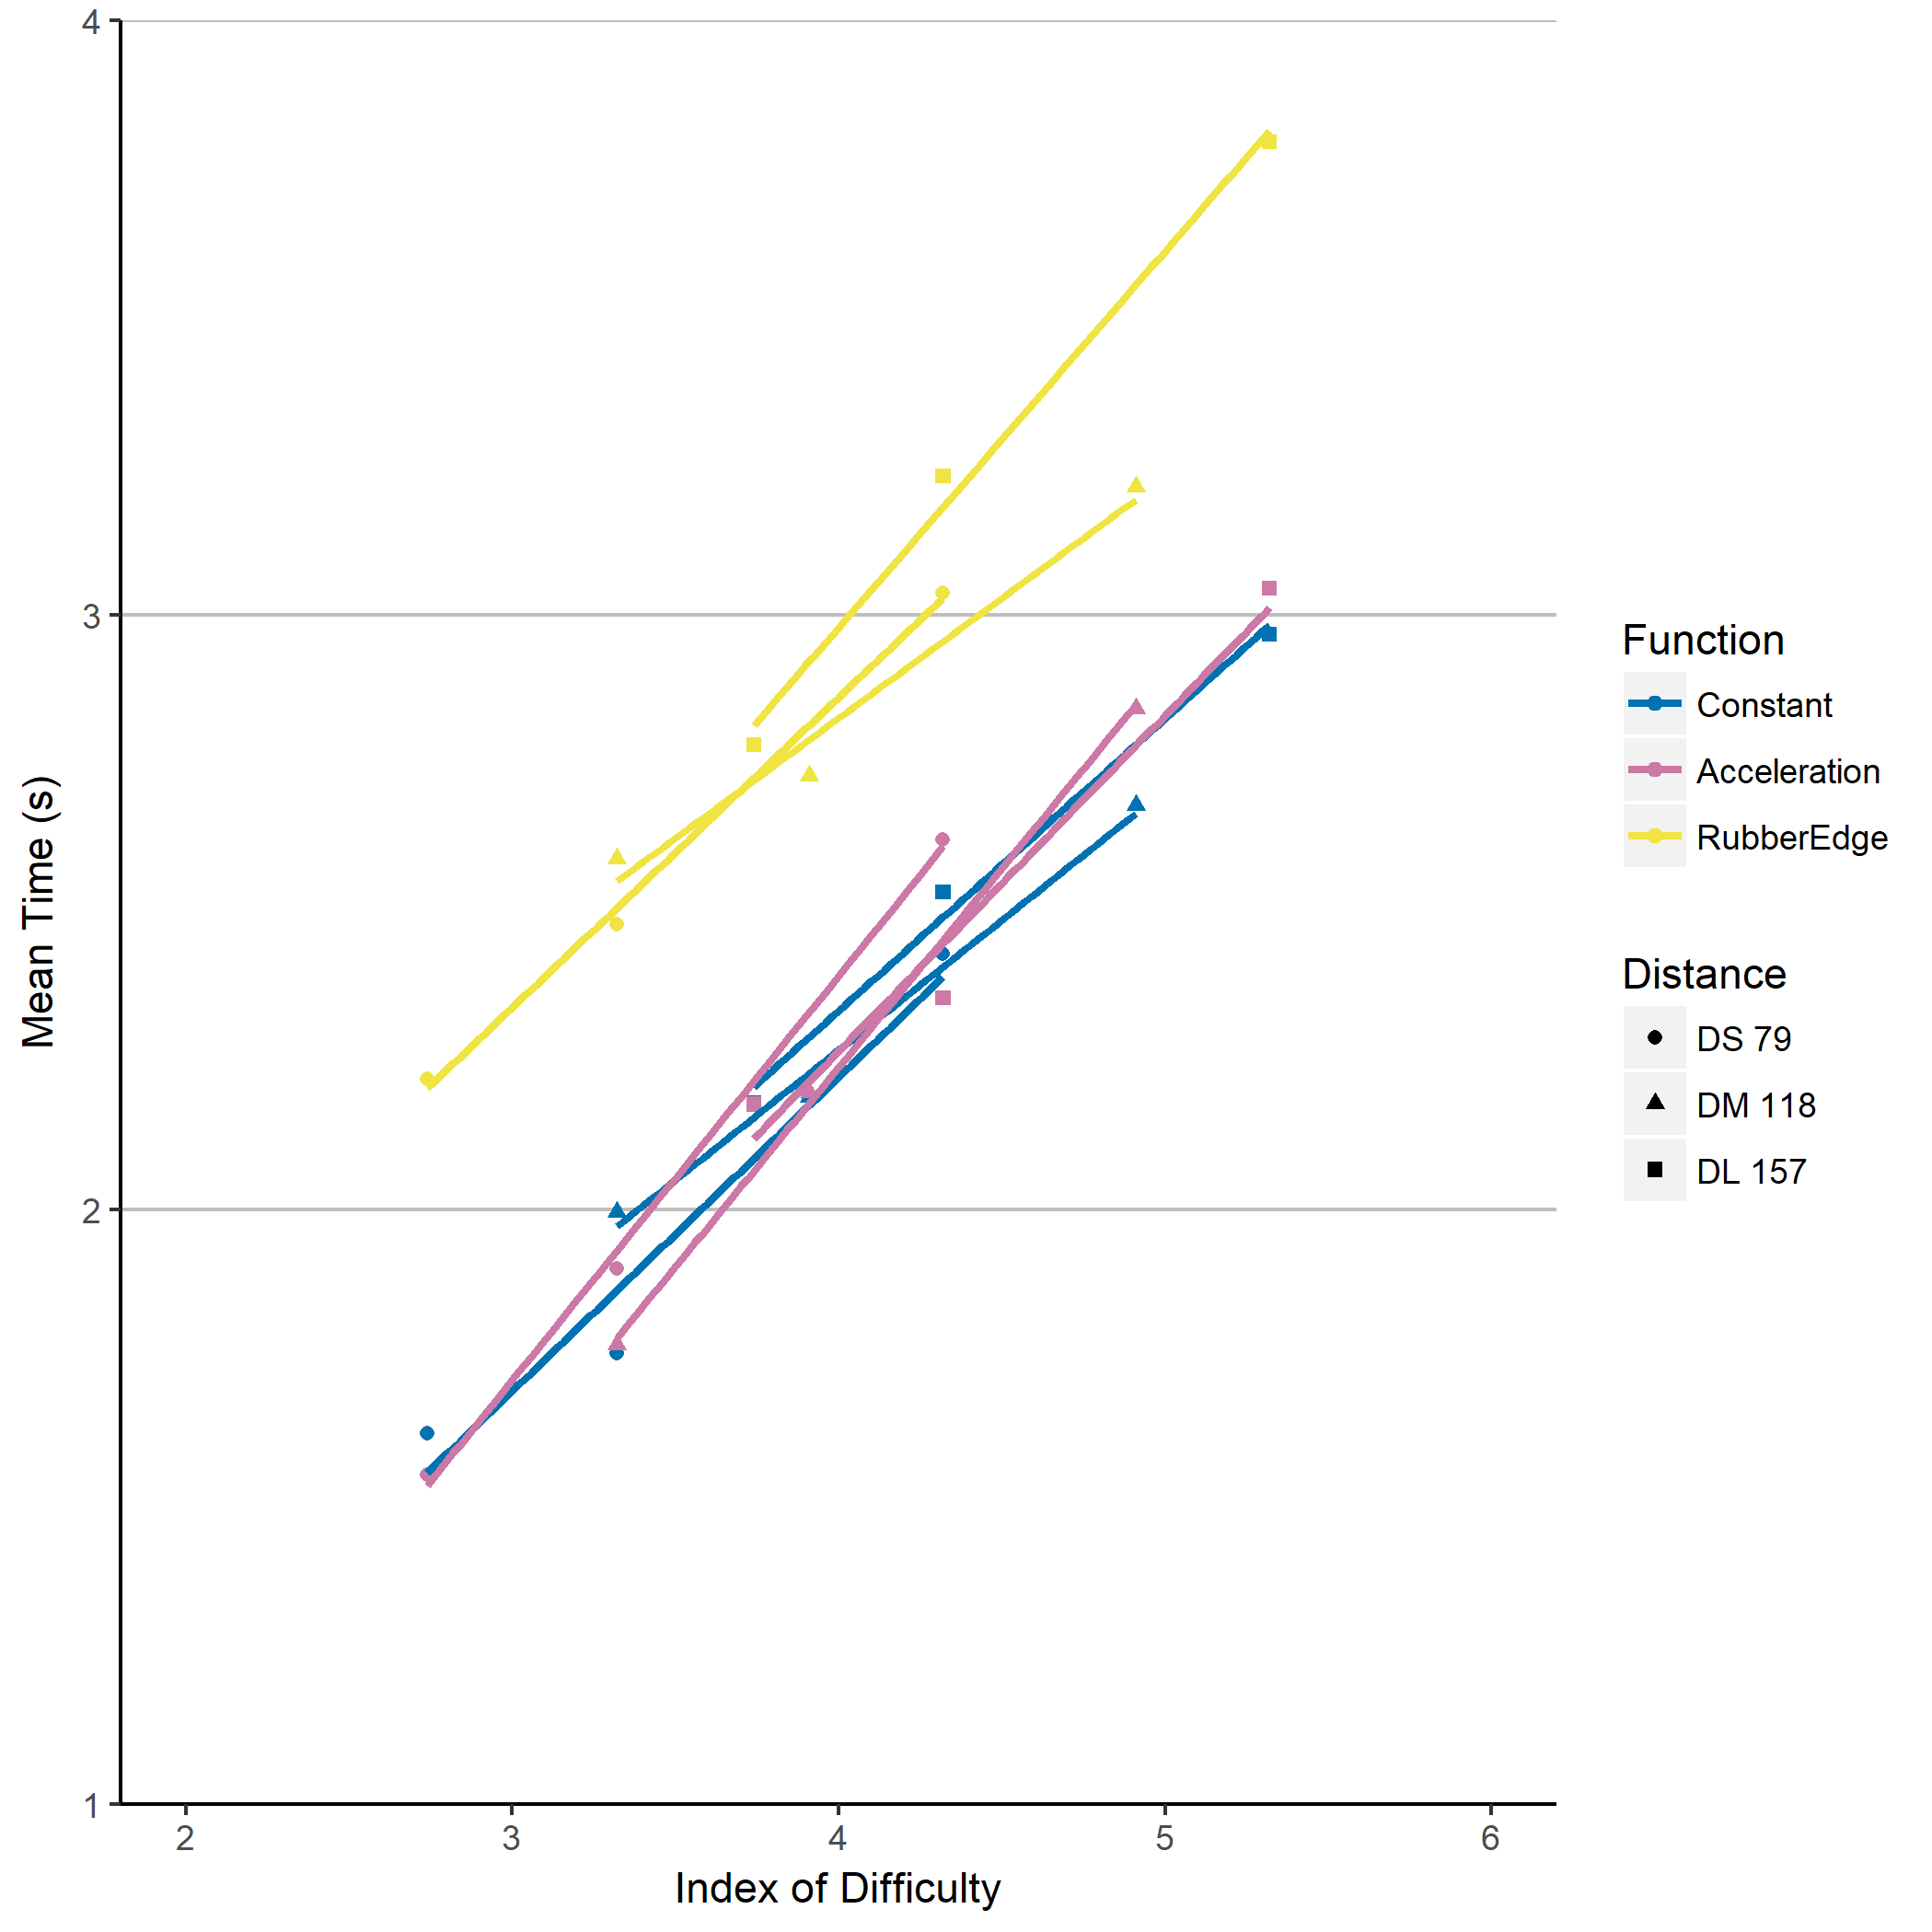
\includegraphics[width=0.9\columnwidth]{fitts-grouped}
    \caption{A comparison between the Index of difficulty and mean time, between different transfer functions, where each distance is separated into its own group.}
    \label{fig:fitts-grouped}
\end{figure}


Table \ref{table:fitts} also shows that the $r^2$ values for each Transfer Function are within acceptable values. For interest, a Figure showing the different distances is also supplied (Figure \ref{fig:fitts-grouped}). This shows that for each Transfer Function the distances are neatly grouped together.

\subsection{Clutches}
Clutches are the number of times a participant removes their finger from the touchpad to continue the task of moving the pointer to a target. This is recorded on a per trial basis.

\begin{figure}[h]
    \centering
    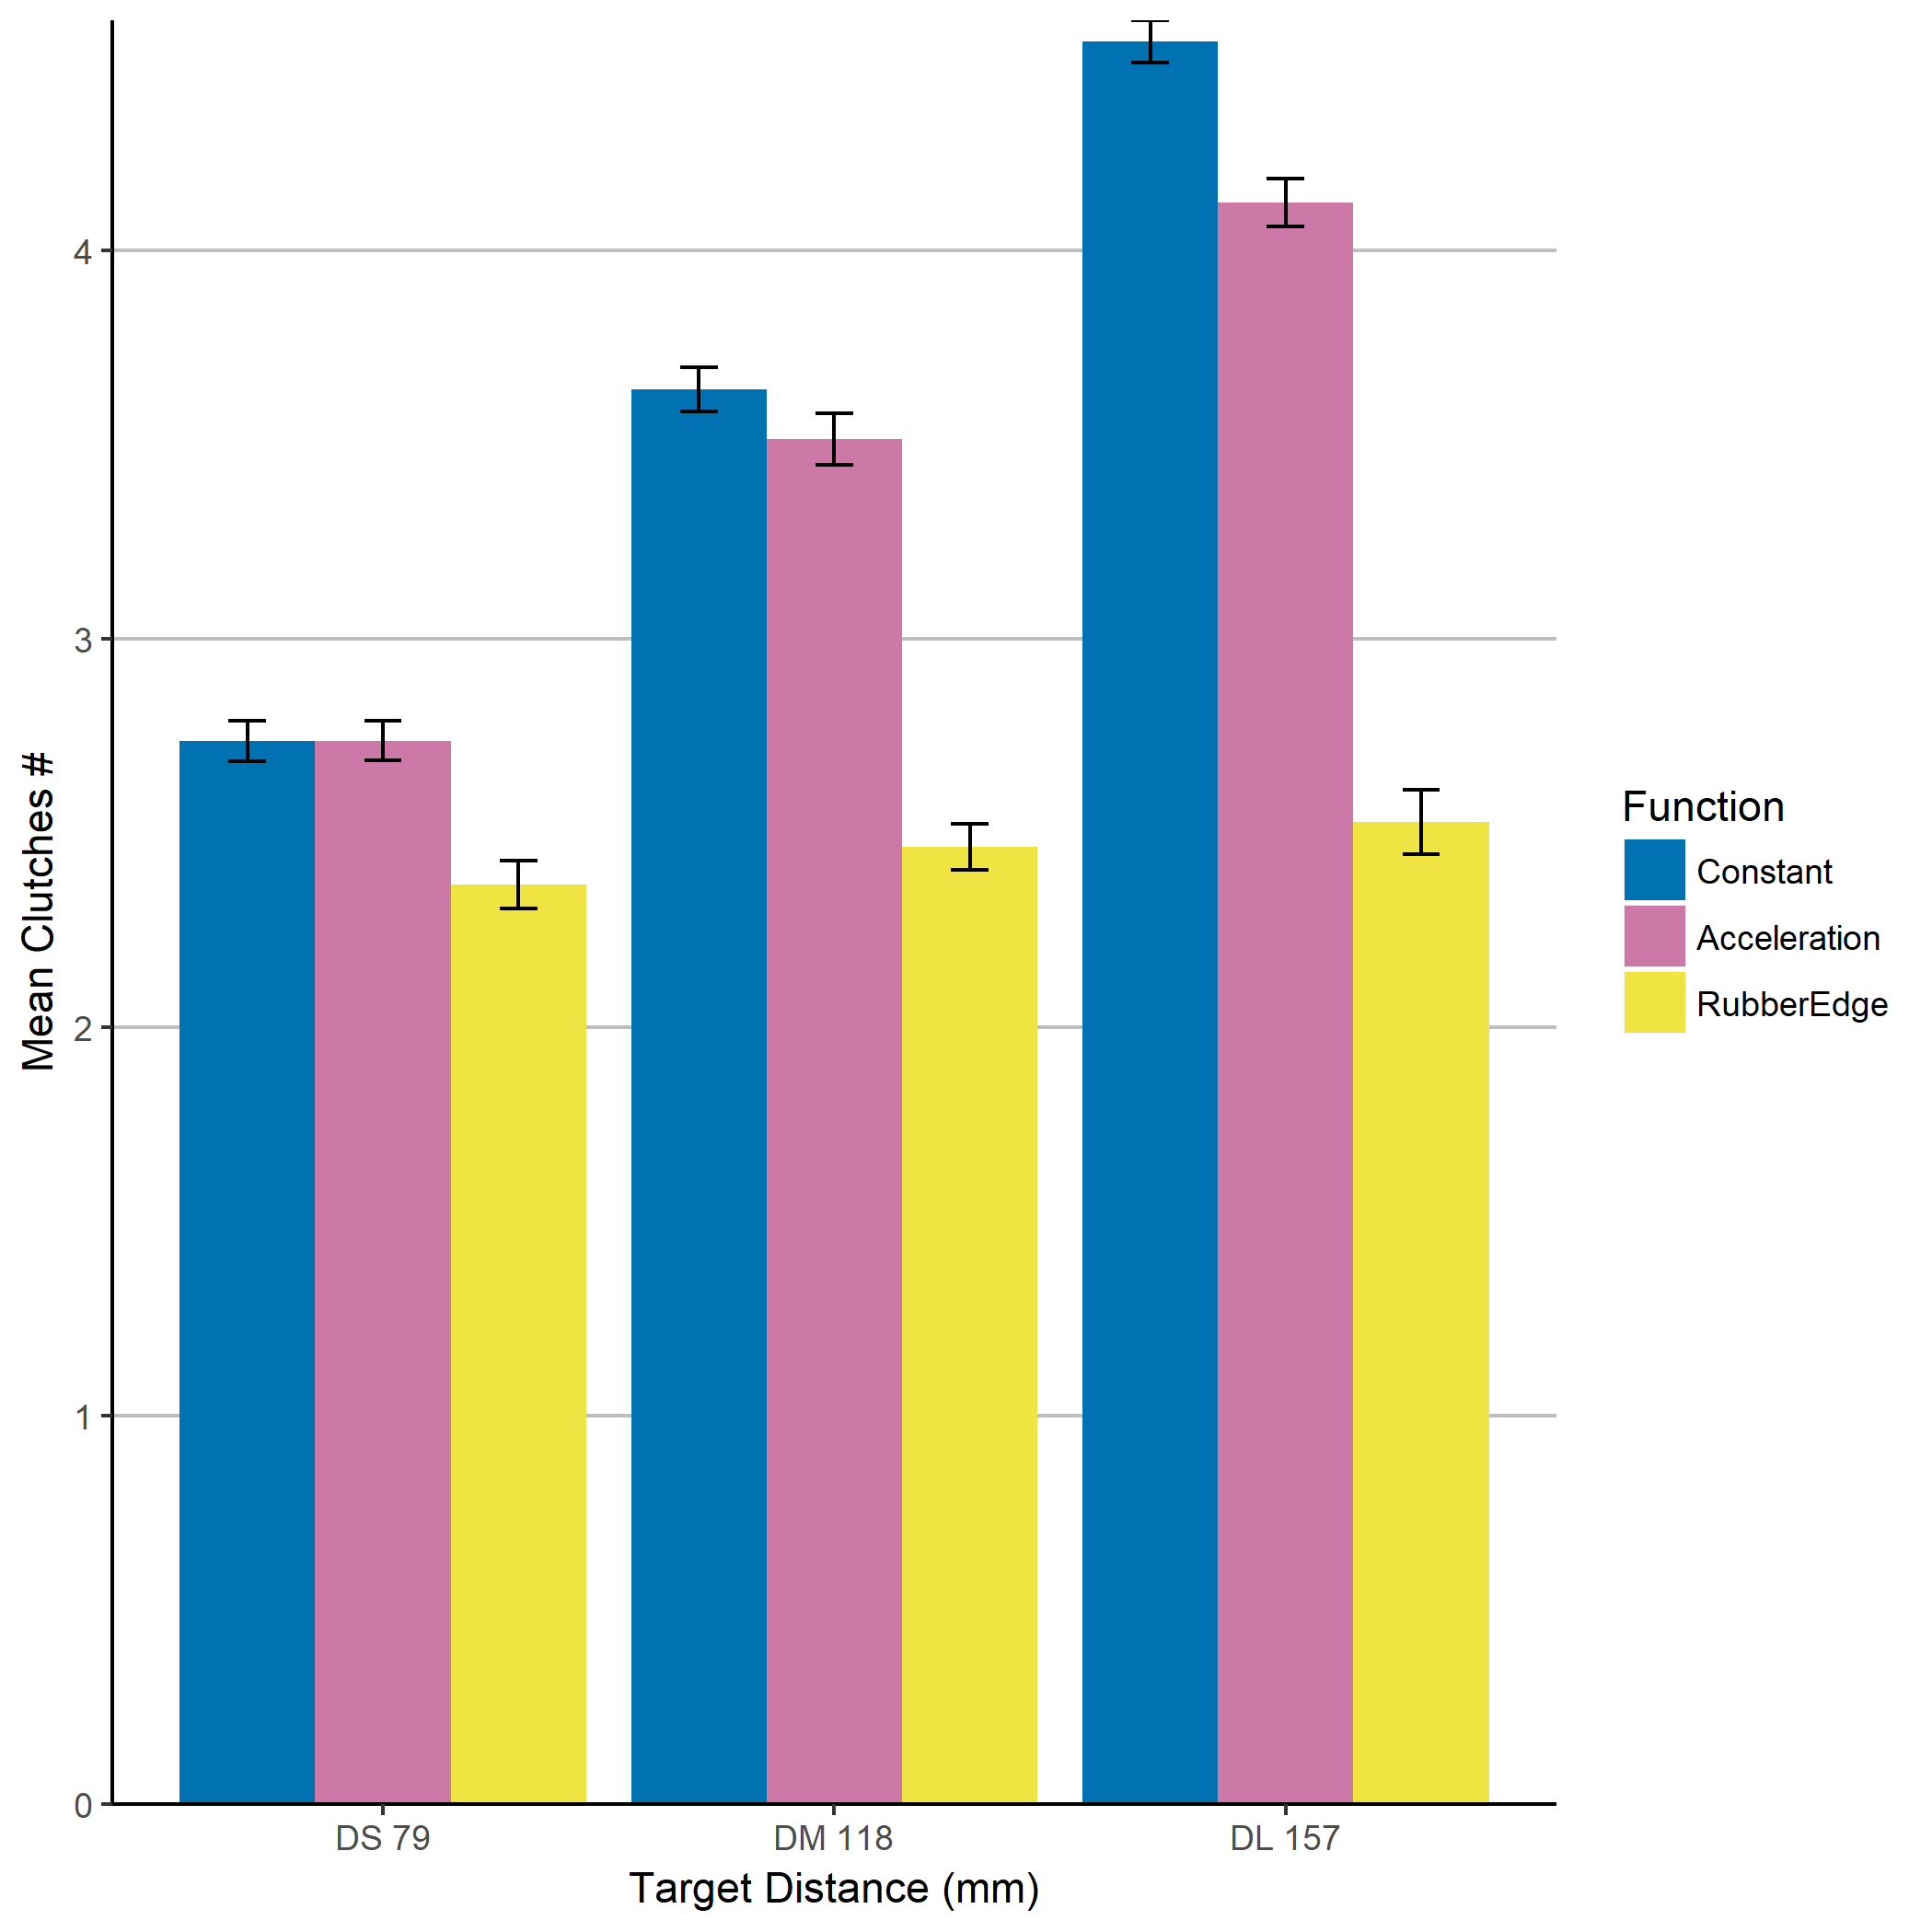
\includegraphics[width=0.9\columnwidth]{clutches}
    \caption{Transfer Function x Distance Interaction on clutch invocations.}
    \label{fig:clutches}
\end{figure}

The order of the Transfer Functions presented to the participants had no significant effect on clutch invocations as found using Mauchly's Test for Sphericity. There was a significant main effect for the Transfer Function on clutch invocations (F$_{2,12}$ = 23.4, p < 0.0001) with the RubberEdge Function outperforming the Constant and Acceleration Function at all Distances. A significant main effect was also present for Distance on clutch invocations (F$_{2,12}$ = 114.2, p < 0.0001). More importantly, there was a significant Transfer Function x Distance interaction (F$_{2,24}$ = 32.2, p < 0.0001), as shown in Figure \ref{fig:clutches}. RubberEdge outperforms both the Constant and Acceleration functions at all Distances (D$_S$, D$_M$, D$_L$) by ~(13.6\%, 31.1\%, 41.6\%) respectively. A pair-wise comparison confirms this finding with both Acceleration vs RubberEdge and Constant vs RubberEdge having p < 0.0001. We therefore accept \textbf{H1}.


\subsection{Participant Feedback}
Participants were asked the following question for each Transfer Function at the end of the experiment. 'Was the interface frustrating to use?', 'Was the interface easy to use?' and 'The interface felt accurate?'. Only the question about accuracy was found to be significant ($x^2_r = 6.42$, df = 2, $p = < 0.05$). Where 5 out of 7 participants agreed that the Constant Transfer Function was accurate, 4 out of 7 agreed that Acceleration was accurate and 4 out of 7 participants found that RubberEdge not to be accurate.

Participants commented the noticeable lag in the pointer see section \ref{section:interface_problems}, which details the issue. 